% !TeX root = ../Book3.tex
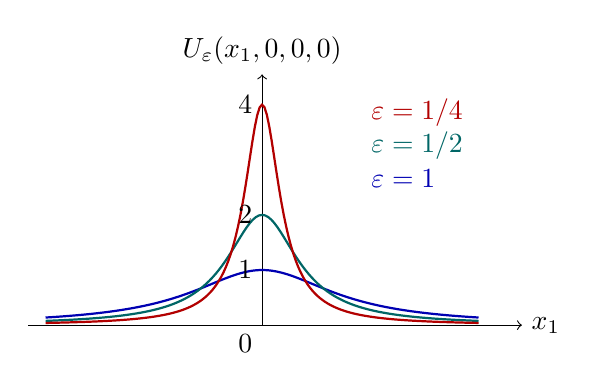
\begin{tikzpicture}[x=1.1cm,y=0.7cm]
	\draw[->] (-2.7,0)--(3.0,0) node[right] {\(x_1\)};
	\draw[->] (0,0)--(0,4.55) node[above] {\(U_\varepsilon(x_1,0,0,0)\)};
	\draw[thick,blue!70!black,domain=-2.5:2.5,samples=141] plot (\x,{1/(1+\x*\x)});
	\draw[thick,teal!80!black,domain=-2.5:2.5,samples=141] plot (\x,{0.5/(0.25+\x*\x)});
	\draw[thick,red!70!black,domain=-2.5:2.5,samples=181] plot (\x,{0.25/(0.0625+\x*\x)});
	\node[left] at (0,1) {\(1\)};
	\node[left] at (0,2) {\(2\)};
	\node[left] at (0,4) {\(4\)};
	\node[blue!70!black,right] at (1.15,2.65) {\(\varepsilon=1\)};
	\node[teal!80!black,right] at (1.15,3.25) {\(\varepsilon=1/2\)};
	\node[red!70!black,right] at (1.15,3.85) {\(\varepsilon=1/4\)};
	\node[below left] at (0,0) {\(0\)};
\end{tikzpicture}
